%!TEX root=report.tex
\subsection{k-means clustering}

\subsubsection{Indentifing the amount of clusters}
Due to the size of the dataset (64800, 341), and the fact multiple simulated datasets of the same size would be needed to calculate the gap-statistic it was calculated in the HPC cluster that DTU offers for students and faculty.
It should be noted that if such a setup haven't been available, one could have used smaller subsamples of the data.
5 simulation samples of size (64800,341) was made using a multivariate uniform distribution. The following is the plot of the resulting gap statistic with its standard deviation.
\begin{figure}[H]
	\center
	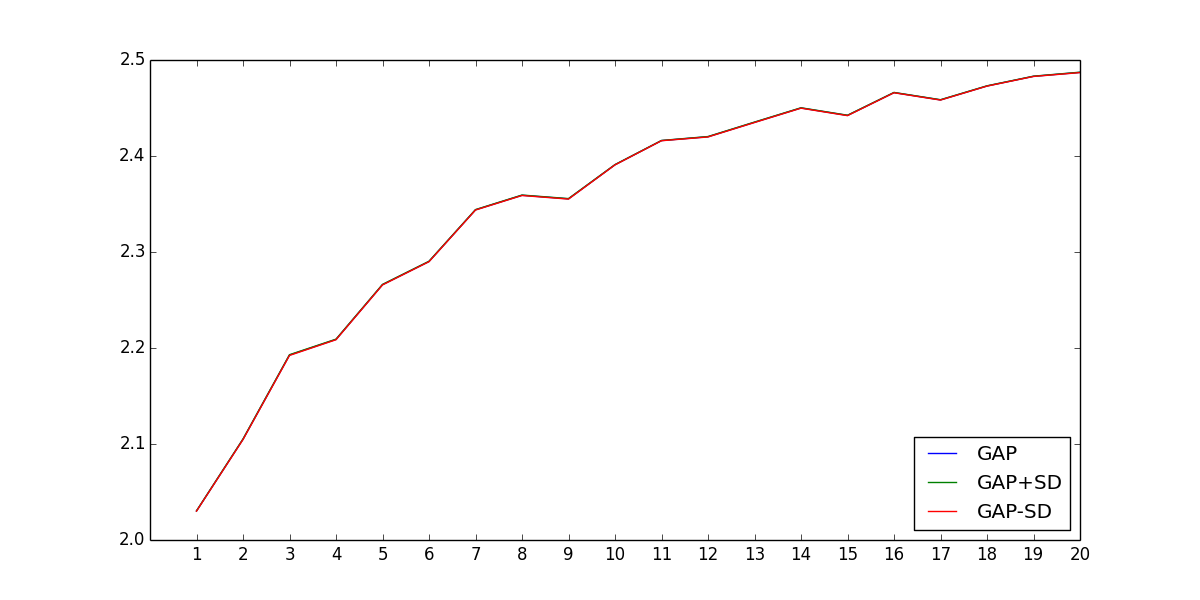
\includegraphics[width=\textwidth]{figures/kmeans-gap.png}
	\caption{Gap statics and standard deviation. It is not an error that the 3 lines overlap; it is simply caused by the large amount of simulation samples which leads to a very small $W_k$ which in turn causes $SD(Log(W_k)$ to be small approximately $10^{-3}$.}
\end{figure}\todo{This makes no sense.}

Based on the gap-statistics one obtains that 8 clusters is the optimal choise. Using 8 cluster, one can color code each cluster in a different color and plot it on the world map, and along side it include a plot of the clusters centroids.

\begin{figure}[H]
	\center
	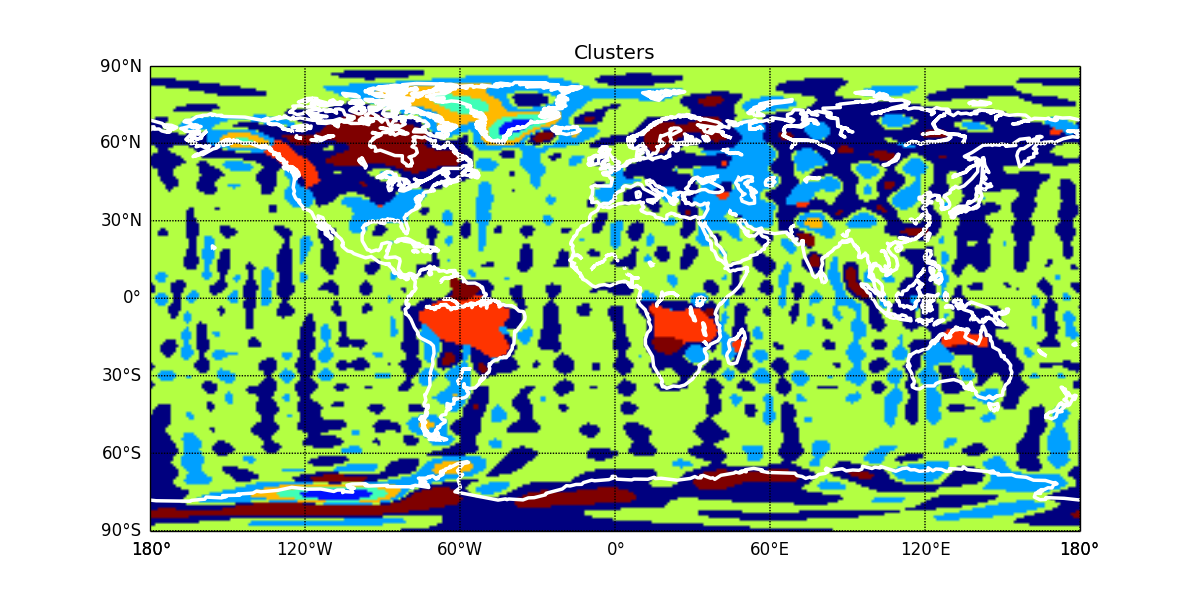
\includegraphics[width=\textwidth]{figures/kmeans-world-clusters}
	\caption{Each position is an point with belongs to the cluster, with the closest centroid.}
	\label{fig:kmeans-world-clusters}
\end{figure}
\begin{figure}[H]
	\center
	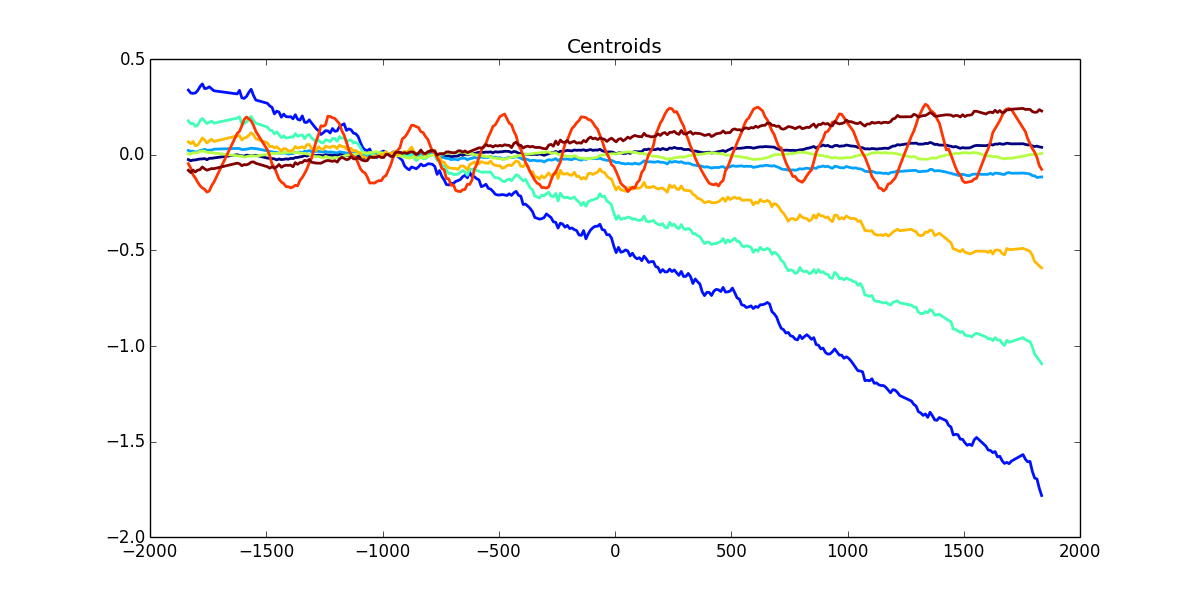
\includegraphics[width=\textwidth]{figures/kmeans-centroids}
	\caption{Cluster centroids. The colors correspond to those in Figure \ref{fig:kmean-world-clusters}}
	\label{fig:kmeans-centroids}
\end{figure}

Comparing the two plot above a few interesting insights are gained:
\begin{itemize}
 \item The ocean are primarily green.
\item Some places though the oceans are either dark blue or light blue. Those two centroid appears to be a kind of specific noise that somehow repeats itself across the globe. This might be artifacts from actual noise in the data.
\item Dark red areas have a slight mass increase. At the south pole it appears that some of the mass loss at the edge actually moves inward towards the South Pole. This may be caused by post glacial rebound as no GIA have been performed.
\item  Bright red correlates with extreme and regular seasonality (i.e. rain season in South America).
\item Orange, teal and blue correspond with trending mass loss. The most significant locations appear to be located around the tip of the South pole along with Greenland's east coast.
\end{itemize} \todo{Update location names, to comform with Allan}
